\documentclass[11pt,usenames,dvipsnames]{beamer}
\usetheme{Madrid}
\usepackage{lmodern}
\usepackage{xcolor}



\usepackage[utf8]{inputenc}
\usepackage[english]{babel}
\usepackage{amsmath}
\usepackage{amsfonts}
\usepackage{amssymb}
\usepackage{graphicx}
\usepackage{tikz}



\setbeamercolor{block title alerted}{fg=Red, bg=Salmon!50!White}
\setbeamercolor{block body alerted}{bg=Salmon!20!White}


\setbeamercolor*{block title example}{fg=black, bg=Goldenrod}
\setbeamercolor{block body example}{bg=Goldenrod!30!White}

\setbeamercolor*{block title}{fg=White, bg=ForestGreen}
\setbeamercolor{block body}{bg=LimeGreen!30!White}

\setbeamertemplate{footline}{
\begin{flushright}
\Large\insertframenumber
\end{flushright}}
\setbeamertemplate{navigation symbols}{}
\author{Presentation by Phil Trommer}
\title{A Machine Learning Perspective on Predictive Coding with PAQ by Knoll \& de Freitas}
%\setbeamercovered{transparent} 
%\setbeamertemplate{navigation symbols}{} 
%\logo{} 
%\institute{} 
%\date{} 
%\subject{} 

% Inserts Section Introduction Slide
\AtBeginSection[] {
	\begin{frame}
		\frametitle{\insertsectionhead}
		\tableofcontents[currentsection,hideothersubsections]
	\end{frame}
}


\newcommand{\defText}[1]{\textcolor{Red}{#1}}





\colorlet{beamer@blendedblue}{ForestGreen}
\begin{document}



\begin{frame}
\titlepage
\end{frame}


\begin{frame}{Overview}
\tableofcontents
\end{frame}


\section{Introduction to PAQ}


\begin{frame}{Introduction to PAQ}
	\begin{block}{What is PAQ8}
			\begin{itemize}
				\item What is it?
				\item How does it work?
				\item What makes it so famous?
			\end{itemize}
	\end{block}
\end{frame}

\begin{frame}{Introduction to PAQ}

	
	\begin{alertblock}{What is PAQ?}<1->
		\begin{itemize}
			\item A lossless, open-source compression algorithm
			\item Brings high perfomance at the cost of increased memory usage and time consumption
			\item Related to PPM, is envisioned as PPMs improvement
		\end{itemize}
	\end{alertblock}
	
		\visible<2->{
	\begin{exampleblock}{Matt Mahoney}
	\begin{minipage}[b]{0.70\linewidth}
		\begin{itemize}
			\item Born 1955
			\item Recieved Ph.D in computer science at Florida Tech in 2003
			\item Released PAQ1 on January 6, 2002
		\end{itemize}
	\hfill
	\end{minipage}
	\begin{minipage}[b]{0.28\linewidth}
		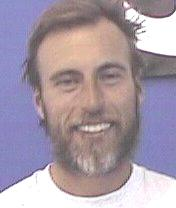
\includegraphics[scale=1.5]{files/matt.jpg}
	\end{minipage}
	\end{exampleblock}
	}
\end{frame}




\begin{frame}{Introduction to PAQ}
	\begin{exampleblock}{Principles of PAQ}
	
		\begin{itemize}
			\item Modeling combined with adaptive arithmetic encoding
			\item Open to additions and improvements
			\item Improves perfomance of PPM by including several predictors (i.e. models of data) 
			\item Combines the result of the predictors
		\end{itemize}
	\end{exampleblock}

\end{frame}

\begin{frame}{Introduction to PAQ}
	\begin{block}{Exemplary Predictors}
	\visible<1->{The order-$n$ context predictor
		\begin{itemize}
			\item Examines the last $n$ bits and counts the 1's and 0's
			\item Estimates probability whether next bit is 1 or 0 like PPM
		\end{itemize}	
		}		
	\visible<2->{
	The sparse context predictor
		\begin{itemize}
			\item 	Context consists of a specific amount of non-contiguous bytes before the current bit
		\end{itemize}
		}
		
	\visible<3->{
	Whole word order-$n$ context
		\begin{itemize}
			\item Context is the latest $n$ whole words
		\end{itemize}
	}
	\end{block}
	

	
\end{frame}


\begin{frame}{Introduction to PAQ}
		\begin{exampleblock}{PAQ \& Predictors}<1->
		\begin{itemize}
			\item PAQ encoder looks at the beginning of input file for deciding which predictors are used
			\item Ways to combine predictions change through with the different versions
			\item Each predictor outputs a pair of bit counts $\left(n_0 , n_1\right)$ 
			\item Counts of each predictor are weighted with context length
		 	\item Those counts get summed up 
		\end{itemize}

	\end{exampleblock}
\end{frame}

\section{PAQ8L}
\begin{frame}{PAQ8L}
	\begin{exampleblock}{PAQ8 - What's new?}<1->
		\begin{itemize}
			\item Predictors don't produce a pair of bit counts anymore\\
			$\hookrightarrow$ those counts get weighted and normalized into the interval $[0,1]\subset\mathbb{R}$
			\item Instead  each predictor already outputs a probability
			\item \textit{paq8l} is a stable version of paq8, released by Matt Mahoney
		\end{itemize}
	\end{exampleblock}
	
		\begin{alertblock}{PAQ8L - Machine Learning Perspective}<2->
		\begin{itemize}
			\item paq8l is the version of PAQ used by \textit{Byron Knoll \& Nando de Freitas}
			\item They try to show the possibilities of PAQ beyond data compression
		\end{itemize}
	\end{alertblock}
\end{frame}

\subsection{Architecture}
\begin{frame}{Architecture}


	\begin{exampleblock}{Architecture of PAQ8}<1->
		\begin{itemize}
			\item Uses weighted combination of predictions from Large number of models
			\item Allows non-contiguous context matches
			\item paq8l uses \textbf{552} prediciton models
			\item Combines the output of them into a single one\\
			$\hookrightarrow$ Passes this through an \textit{adaptive probability map} (APM) before using the arithmetic coder
		\end{itemize}
	\end{exampleblock}
	\hfill
	
	\visible<2->{
	\begin{figure}[H]
		\centering
		\resizebox{0.95\textwidth}{!}{
			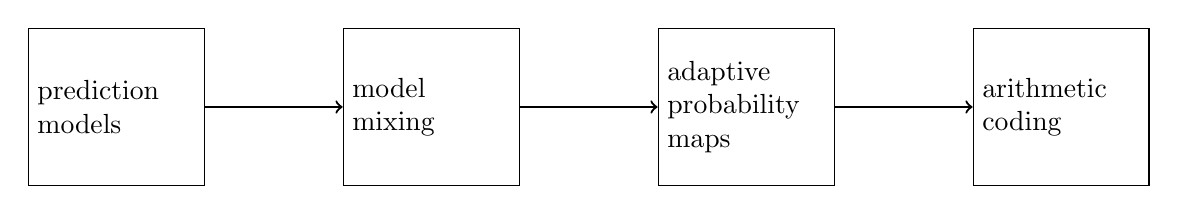
\begin{tikzpicture}[]
	\node[rectangle,draw,minimum height=2cm,text width=2cm] (predModel) at (0,0) {prediction models};
	\node[rectangle,draw,text width=2cm,minimum height=2cm] (modelMix) at (4,0) {model \\ mixing};
	\node[rectangle,draw,text width=2cm,minimum height=2cm] (apm) at (8,0) {adaptive probability maps};
	\node[rectangle,draw,text width=2cm,minimum height=2cm] (arithCoding) at (12,0) {arithmetic coding};

\draw[->,thick](predModel) -- (modelMix);
\draw[->,thick](modelMix) -- (apm);
\draw[->,thick](apm) -- (arithCoding);

\end{tikzpicture}
		}
		\caption{PAQ8 Architecture}
	\end{figure}
	}

	

\end{frame}

\subsection{Neural Network}
\begin{frame}{Neural network}
		
	\begin{alertblock}{Neurons of a neural network}<1->
	A \defText{neuron} takes one or more \defText{inputs} and gives an \defText{output}. \\
	Within the topic of machine learning, the neuron can be understood as a \defText{function}.
	\end{alertblock}

	\visible<2->{
		\begin{figure}[H]
			\centering
			\resizebox{0.275\textwidth}{!}{
				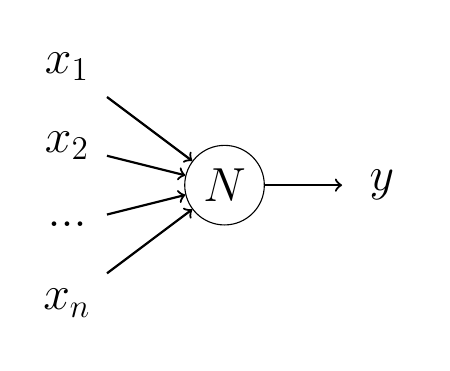
\begin{tikzpicture}[]
	\node[circle,draw,minimum size=1cm] (n) at (2,1.5) {\LARGE$N$};
	\node[minimum size=1cm] (x1) at (0,3) {\LARGE$x_1$};
	\node[minimum size=1cm] (x2) at (0,2) {\LARGE$x_2$};
	\node[minimum size=1cm] (xdot) at (0,1) {\LARGE$...$};
	\node[minimum size=1cm] (xn) at (0,0) {\LARGE$x_n$};
	\node[minimum size=1cm] (y) at (4,1.5) {\LARGE$y$};

\draw [->,thick](x1) -- (n);
\draw[->,thick] (x2) -- (n);
\draw[->,thick] (xdot) -- (n);
\draw[->,thick] (xn) -- (n);
\draw[->,thick] (n) -- (y);
	







\end{tikzpicture}
			}
			\caption{Neural network architecture}
		\end{figure}
	}
	

		
	
\end{frame}




\begin{frame}{Neural network}

	\begin{alertblock}{Layer in neural network}<1->
			A layer is a group of neurons.
	\end{alertblock}	
	
		
		
	\visible<2->{
	\begin{alertblock}{A neural network}
	Neural networks is defined by its layers:
	\begin{itemize}
		\item 1 input layer with $n$ inputs 
		\item 1 output layer with $k$ outputs
		\item $M$ layers between input and output layer (i.e. hidden layers)
		\item Layers can consist of different amounts of neurons
	\end{itemize}
	\end{alertblock}	
	
	}	
	
	\visible<3->{
	
	\begin{block}{General structure of neural network}
		Let it be an generic neural network with:	
		\begin{itemize}
			\item $x_1,...x_n$ inputs and $y_1,...,y_k$ outputs
			\item There are $M$ different layers between input and output
		\end{itemize}
	\end{block}
	}	

	
	


\end{frame}

\begin{frame}{Neural network}
		%Change picture to just a neuron
	\visible<1->{
	\begin{figure}[H]
		\centering
		\resizebox{!}{5cm}{
			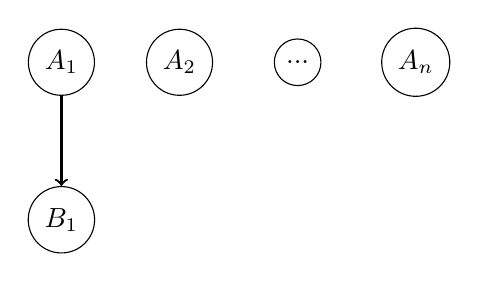
\begin{tikzpicture}[]
	\node[circle,draw] (a1) at (0,0) {$A_1$};
	\node[circle,draw] (a2) at (1.5,0) {$A_2$};
	\node[circle ,draw] (adot) at (3,0) {$...$};
	\node[circle,draw] (an) at (4.5,0) {$A_n$};
	\node[circle,draw] (b1) at (0,-2) {$B_1$};

\draw [->, thick](a1) -- (b1);

\end{tikzpicture}
		}
		\caption{Neural network architecture}
	\end{figure}
	}
\end{frame}


\subsection{Model Mixer}
\begin{frame}{Model Mixer}
	\begin{exampleblock}{Model Mixer of paq8l}<1->
		\begin{itemize}
			\item Resembles a neural network with one hidden layer
			\item One hidden layer is between input and output layer
			\item Subtle differences from a standard neural network
		\end{itemize}
	\end{exampleblock}
	
	\begin{block}{Differences between paq8l and neural networks}<2->
		\begin{enumerate}
			\item Weights for first and second layers are learned online and independently for all nodes:
			\begin{itemize}
				\item Each node trained separately 
				\item reduces predictive cross-entropy error (unlike back propagation)
			\end{itemize}	
			\item Hidden nodes are partitioned into seven sets		 
		\end{enumerate}
	\end{block}
\end{frame}

\begin{frame}{Model Mixer}
	\begin{exampleblock}{Hidden Node Partitioning}
		\begin{itemize}
			\item For every bit of data 1 node from each set
			\item Only edges of selected nodes are updated
			\item $552\times 7 = 3,864$ weights updated per bit
		\end{itemize}
	\end{exampleblock}

		\visible<1->{
		\begin{figure}[H]
			\centering
			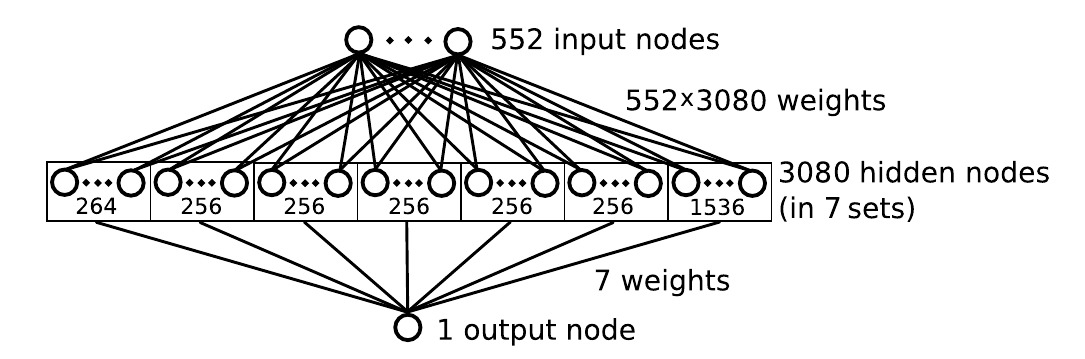
\includegraphics[scale=0.4]{files/model-mixer_architecture.png}
			\caption{Model Mixer architecture  (Graphic by Knoll \& De Freitas)}
		\end{figure}
	}
\end{frame}

\begin{frame}{Model Mixer}
	\begin{block}{Node selection}
		\begin{itemize}
			\item Sets 1,2,4 and 5 choose node based on single byte in context
			\item Set 6 chooses based on length of longest context matched
			\item Sets 3 and 7 use combination of several bytes
			\item Depending on the context, a specific node is selected
		\end{itemize}
	\end{block}
	
	\visible<2->{
	\begin{exampleblock}{Mixtures of Experts}
		\begin{itemize}
			\item Technique published by \textit{Jacobs et al. 1991}
			\item Used for neural network training
			\item Requires a gating network to select expert model
		\end{itemize}
	\end{exampleblock}
	}
\end{frame}


\subsection{Adaptive Probability Maps}
\begin{frame}{Adaptive Probability Maps}
	\begin{alertblock}{Definition APM}
		\begin{itemize}
			\item Takes prediction from model mixer
			\item is an two dimensional table and low order context as input
			\item Outputs a new prediction on non-linear scale
			\item Table entries adjusted after each bit is coded
		\end{itemize}
	\end{alertblock}

\end{frame}

\section{Applications for PAQ8}
\begin{frame}{Classification}
	\begin{exampleblock}{Classification as the basic principle}
		\begin{itemize}
			\item Compression based classification discovered by researches (Marton et al., 2005)
			\item Standard procedures for compression based classification exists
			\item SMDL, AMDL \&  BCN 
		\end{itemize}
	\end{exampleblock}
	
	\visible<2->{
	\begin{alertblock}{Classification procedures}
		\begin{itemize}
			\item \textbf{SMDL} $\rightarrow$ uses differences between test dictionary and result dictionary
			\item \textbf{AMDL \& BCN} $\rightarrow$ uses difference between compressed file sizes (training files \& test file)
		\end{itemize}
	\end{alertblock}	
	} 

\end{frame}

\begin{frame}{Applications for PAQ8}
	\begin{block}{What applications?}
	PAQ8 is useful even beside compressing files.
	\begin{itemize}
		\item Adaptive Text Prediction
		\item Text categorization
		\item Shape recognition
		\item Lossy compression (i.e. JPEG)
	\end{itemize}
	Results are calculated by an module called \textit{PAQclass}
	\end{block}
	\visible<2->{
		\begin{exampleblock}{Adaptive Text Prediction}
			\begin{itemize}
				\item PAQ8 can be used to find string $x$ for some training string $y$
				\item Can be set to work in speech recognition and text prediction (for typing)
			\end{itemize}
		\end{exampleblock}
	}

\end{frame}

\begin{frame}{Text categorization}
		\visible<1->{
		\begin{figure}[H]
			\centering
			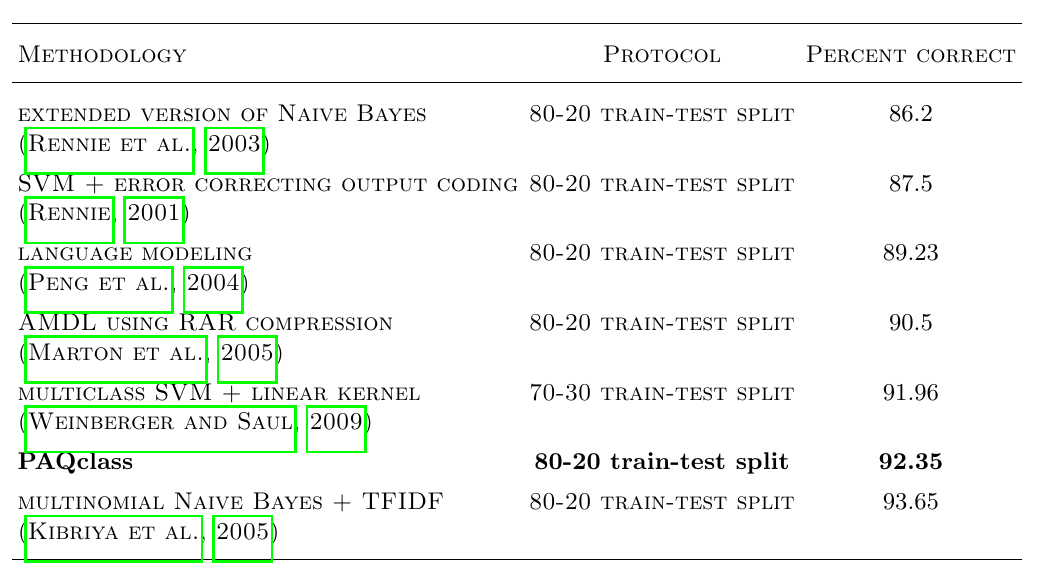
\includegraphics[scale=0.4]{files/text-categorization.png}
			\caption{Text categorization comparison  (Graphic by Knoll \& De Freitas)}
		\end{figure}
	}
\end{frame}

\begin{frame}{Shape recognition}

	\visible<1->{
		\begin{figure}[H]
			\centering
			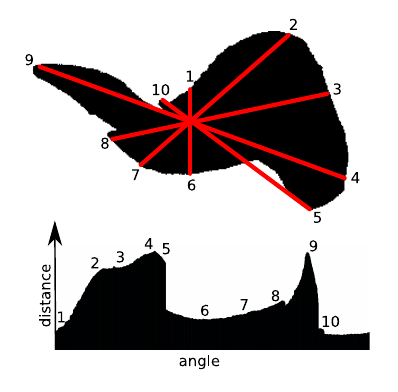
\includegraphics[scale=0.4]{files/shape-recognition.png}
			\caption{Shape recognition principle  (Graphic by Knoll \& De Freitas)}
		\end{figure}
	}

\end{frame}

\begin{frame}{Shape recognition}

	\visible<1->{
		\begin{figure}[H]
			\centering
			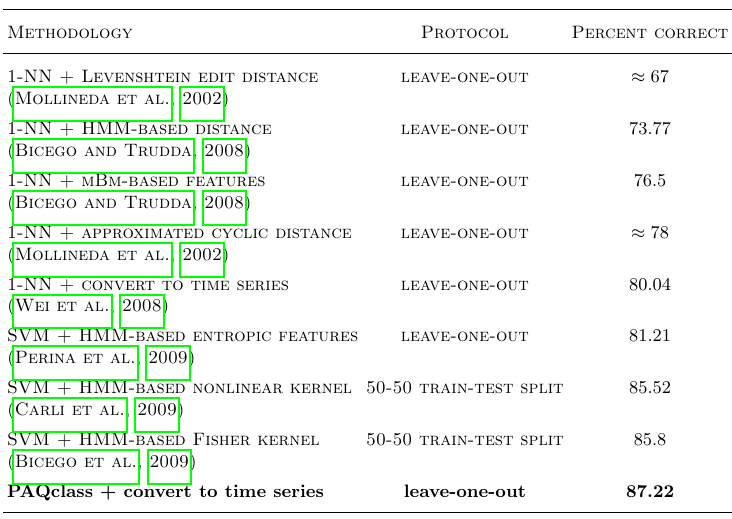
\includegraphics[scale=0.45]{files/shape-recognition-comparison.png}
			\caption{Shape recognition comparison  (Graphic by Knoll \& De Freitas)}
		\end{figure}
	}

\end{frame}

\begin{frame}{Lossy compression}

	\visible<1->{
		\begin{figure}[H]
			\centering
			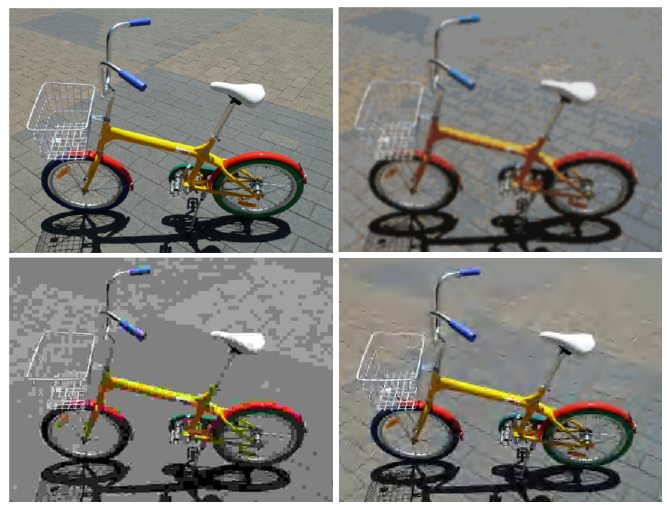
\includegraphics[scale=0.3]{files/picture_compression.png}
			\caption{Picture compression comparison  (Graphic by Knoll \& De Freitas)}
		\end{figure}
		\centering
		\begin{tabular}{l|l}
		Upper-Left: uncompressed & Upper-Right: compressed by paq8\\ 
		700x525 pixel & 4083 bytes\\\hline
		Bottom-Left: JPEG & Bottom-Right: JPEG2000 \\
		16783 bytes & 4097 bytes
		\end{tabular}

	}

\end{frame}

\section{References}

\begin{frame}{References}

\begin{itemize}
	\item \textit{A Machine Learning Perspective on Predictive Coding with PAQ}, Byron Knoll \& Nando de Freitas,
	2019/08/17
	\item https://stackoverflow.com/questions/41990250/what-is-cross-entropy
	\item http://mattmahoney.net/
	\item https://www.techopedia.com/definition/33264/hidden-layer-neural-networks
	\item \textit{Handbook of Datacompression}, 5th Edition, Springer
\end{itemize}

\end{frame}



\end{document}